% !TeX spellcheck = en_GB
\documentclass[10pt,letterpaper,oneside]{article}
\usepackage{fontspec}
\usepackage{arev}
\usepackage[utf8]{inputenc}
\usepackage[T1]{fontenc}
\usepackage{amsmath}
\usepackage{amsfonts}
\usepackage{amssymb}
\usepackage{graphicx}
\usepackage{csquotes}
\usepackage{booktabs}
\usepackage{multicol}
\usepackage{enumerate}
\usepackage{microtype}
\usepackage[labelfont=bf,font={small}]{caption}
\usepackage{hyperref}
\usepackage{booktabs}
\usepackage{subcaption}
\usepackage{fancyhdr}
\usepackage[svgnames]{xcolor}
\usepackage{mdframed}
\usepackage{multicol}
\usepackage[para]{footmisc}
\usepackage{siunitx}
\usepackage{cleveref}
\usepackage{listings}
\usepackage{cprotect}


\lstset{ % General setup for the package
	language=Python,
	basicstyle=\small\ttfamily,
	tabsize=4,
	columns=fixed,
	showstringspaces=false,
	showtabs=false,
	keepspaces,
	commentstyle=\color{SeaGreen},
	keywordstyle=\bf\ttfamily\color{DarkBlue}
}

\newfontfamily\symbolfont{Symbola}
\usepackage[left=1in,right=1in,top=1in,bottom=1in,marginparwidth=0.3in]{geometry}

\usepackage[sorting=none]{biblatex}
\addbibresource{../bibliography.bib}

\author{Andreas Stöckel\\[0.5cm]Based on lecture notes by\\Chris Eliasmith and Terrence~C.~Stewart}
\newcommand{\baseCodeURL}{https://github.com/astoeckel/syde556-w20/blob/master/lectures}

\fancyhf{}
\fancyhead[L]{SYDE 556/750 Lecture Notes}
\fancyhead[R]{Andreas Stöckel}
\fancyfoot[C]{\thepage}
\pagestyle{fancy}

\setlength{\parindent}{0em}
\setlength{\parskip}{0.5em}
\renewcommand{\baselinestretch}{1.25}
\renewcommand{\vec}[1]{{\mathbf{#1}}}
\newcommand{\mat}[1]{{\mathbf{#1}}}
\newcommand{\T}{\ensuremath{\mathrm{T}}}
\renewcommand{\epsilon}{\varepsilon}
\renewcommand{\phi}{\varphi}

\makeatletter
\newcommand{\superimpose}[2]{%
	{\ooalign{{#1}\hidewidth\cr{#2}\hidewidth\cr}}}
\makeatother
\newcommand{\SolidCircle}[2]{\superimpose{\color{#1}\symbolfont ⬤}{\textbf{\color{white}#2}}\hspace{1em}}
\newcommand{\OPlus}{\SolidCircle{DarkGreen}{\kern0.75pt+}}
\newcommand{\OMeh}{\SolidCircle{DarkOrange}{~}}
\newcommand{\OMinus}{\SolidCircle{DarkRed}{\kern2.25pt--}}

\newcommand{\YouTube}[2][Video]{\href{https://youtu.be/#2}{{\symbolfont 📺}~{#1}}%
%\footnote{\url{https://youtu.be/#2}}%
}

\newcommand{\CodeLink}[2][Code]{\href{\baseCodeURL/#2}{{\symbolfont ⌨}~\emph{#1}}}

\newcommand{\MakeTitle}[1]{
\maketitle
\begin{center}
	
\includegraphics[width=0.5\textwidth]{../assets/uwlogo.pdf}\\[1cm]
	{#1}\
\end{center}

\vfill

\thispagestyle{empty}
\setcounter{page}{0}
\newpage

\pagenumbering{roman}
\setcounter{tocdepth}{2}
\tableofcontents
\newpage

\setcounter{page}{0}
\pagenumbering{arabic}}

\reversemarginpar


\newcommand{\ColorBox}[3]{%
	\marginpar{%
		\huge\raisebox{-3ex}{\symbolfont{#1}}%
	}%
	\begin{mdframed}[hidealllines=true,backgroundcolor=#2,innertopmargin=0.25cm,innerbottommargin=0.25cm]%
		{#3}
	\end{mdframed}}

\newcommand{\Note}[1]{\ColorBox{📌}{WhiteSmoke}{\textbf{Note:} #1}}
\newcommand{\Example}[1]{\ColorBox{💡}{WhiteSmoke}{\textbf{Example:} #1}}
\newcommand{\Aside}[1]{\ColorBox{🌟}{WhiteSmoke}{\emph{Aside:} #1}}
\newcommand{\Python}[1]{\ColorBox{🐍}{WhiteSmoke}{#1}}
\newcommand{\Notation}[1]{\ColorBox{\huge$\Sigma$}{WhiteSmoke}{\textbf{Notaton:} #1}}

\newcommand{\ConstructionSite}{\hrulefill {\symbolfont 🚧} UNDER CONSTRUCTION {\symbolfont 🚧} \hrulefill}

\newenvironment{ImportantEqn}[1]{\mdframed\raggedleft\emph{({#1})}\align}{\endalign\endmdframed}

\date{January 30, 2020}
\title{SYDE 556/750 \\ Simulating Neurobiological Systems \\ Lecture 5: Feed-Forward Transformation}


\begin{document}
	
	\MakeTitle{\textbf{Accompanying Readings: Chapter 6 of Neural Engineering}}
	
	\section{Introduction}
	
	\Note{Until now, we have been concerned with \emph{representation} in individual populations of neurons. However, we ultimately want to be able to build neural \emph{networks}. This means that we have to find a systematic way of connecting neural populations. Optimally, the connections should be chosen in such a way that information represented in the populations is \emph{transformed} in a useful way.}
	
	We postulated that groups of neurons represent $d$-dimensional quantities $\vec x$ using nonlinear encoding. The encoding process can be further separated into two stages: translating an input $\vec x$ into a per-neuron input current $J_i$ and applying the neural nonlinearity.
	
	The current $J_i$ that is being injected into the $i$-th neuron of a population is defined as
	\begin{align}
	J_i &= \alpha_i \langle \vec e_i, \vec x \rangle + J^\mathrm{bias}_i \,.
	\label{eqn:current}
	\end{align}
	For rate neurons, this input current is turned into a spike rate according to the rate approximation $a_i = G[J_i]$. In the context of spiking neurons, the input current is translated into a spike train $a_i(t)$, a sum of Dirac-$\delta$ pulses.
	
	We further postulated that the value being represented by a population can be estimated using a linear decoder $\mat D$. For spiking neurons, we added a filtering step using a filter $h$
	\begin{align}
	\hat{\vec x} &= \mat D \vec a \quad \text{ for rate neurons,} & 
	\hat{\vec x}(t) &= \big( (\mat D \vec a(t)) \ast h \big)(t) \quad \text{ for spiking neurons.}
	\label{eqn:decoding}
	\end{align}
	
	\Note{\emph{Decoder computation.} We discussed two methods for computing decoders $\mat D$.
		
		For the first method, we generated a random set of samples arranged in a matrix $\mat X$. Using the spike rate approximation $G[J]$, we computed an activity matrix $\mat A$ and obtained $\mat D$ using the solution to the $L_2$-regularised least-squares problem
		\begin{align*}
		\mat D^T = (\mat A \mat A^T + N \sigma^2 \mat I)^{-1} \mat A \mat X^T \,,
		\end{align*}
		where we estimate $\sigma$ to match the deviation between the spike rate estimate and the actual spike rates occurring in the network.
		
		The second solution was to use a random input function $\vec x(t)$, and the recorded (filtered) population spike trains $\vec a(t)$. We  discretised these functions into matrices $\mat A$ and $\mat X$ and used the unregularised solution to the least-squares problem to obtain $\mat D$
		\begin{align*}
		\mat D^T = (\mat A \mat A^T)^{-1} \mat A \mat X^T \,.
		\end{align*}
		
		As mentioned in the last lecture, these two methods should result in approximately the same decoders. While the second method is technically superior, as it accurately characterises the noise present in the neural population, the first method is computationally much cheaper. This is why -- from now on -- we will use the first method to compute the decoders. We can then use this decoding matrix in conjunction with spiking neurons.}
	
	
	Of course, just describing an individual population of neurons is not really useful when building large-scale brain models. We ultimately would like to describe how information is \emph{transformed} while it is sent from one population of neurons to another. In the Neural Engineering Framework, connections between neural populations are performing these transformations.
	\begin{mdframed}
		\textbf{NEF Principle 2 -- Transformation}\\
		Connections between populations describe transformations of neural representations. These transformations are functions of the variables that are represented
		by neural populations.
	\end{mdframed}
	
	When looking at transformations from the perspective of large-scale modelling, researchers are usually confronted with two very different questions.
	\begin{itemize}
		\item \textbf{How do brains \emph{learn} transformations?}
		In other words, how are the connection weights between neuron populations formed in such a way during the lifetime of an animal that they implement a desired task.
		\item \textbf{What are \emph{optimal} connection weights that compute a certain transformation?}
		Here, we assume that a brain has already learned to optimally perform a certain task. In that case, we would just like to know what the corresponding connection weights the system could have learned are. We would then like to use these weights in our model. Essentially, we are building a model of a system that is already an expert.
	\end{itemize}
	For now, we will mostly concern ourselves with the second question, i.e.,~we are trying to build models of \enquote{adult} or \enquote{expert} systems already capable of solving a certain task. We postulate what the transformation may be that the system has learned and compute the optimal weights that implement this transformation. We will talk about \emph{learning}, i.e.,~building a system that learns connection weights while it is being executed in a later lecture.

	\Note{\emph{Hypothesis generation and testing.}
		We should pause here and wonder what the scientific purpose of building neural models with optimal connection weights is. Especially since we do not assume that the brain itself employs the techniques for computing function decoders we discuss below. So, if not providing a theory of how synaptic weights are formed within brains, what is the purpose of the Neural Engineering Framework?
	
		Most importantly, the Neural Engineering Framework can be used to test hypotheses regarding potential functions of neurobiological systems. That is, we can test whether such a system could implement a certain function \emph{under optimal circumstances}. Conversely, if we are not able to implement a function using mathematically optimal connection weights (but taking other constraints into account), we can rule out this hypothesis.

		Furthermore, building working functional models of neural systems remains challenging, even under the \enquote{optimal synaptic weights} assumption. Hence, the Neural Engineering Framework is not only an important tool for testing hypotheses (\enquote{can a function in theory be implemented in a certain way?}), but also for explorative generation of hypotheses (\enquote{this works within the NEF, could the brain be doing this?}).}

	\section{Building a Communication Channel}
	
	The simplest possible transformation is the identity function. Assume that we have two neural populations $A$ and $B$, where $A$ represents a $d$-dimensional vector $\vec x \in \mathbb{R}^{d}$ using $n$ neurons, and $B$ represents a vector $\vec y \in \mathbb{R}^{d'}$ using $m$ neurons. We would now like to send the value $\vec x$ from $A$ to $B$ (assuming that $d = d'$), such that when simulating the network $\vec x$ and $\vec y$ are approximately the same at all times. This type of transformation is also called a \emph{communication channel}, since we are merely sending information from one point in the system to another point in the system without altering it.

	Let's try to think about how to build a communication channel \enquote{computing} $\vec y = \vec x$ in a biologically plausible neural network. Then, in the next section, we will take what we have learned and apply it to arbitrary transformations $\vec y = f(\vec x)$.
	
	\subsection{Sequential Decoding and Encoding}
	
	\begin{figure}[p]
		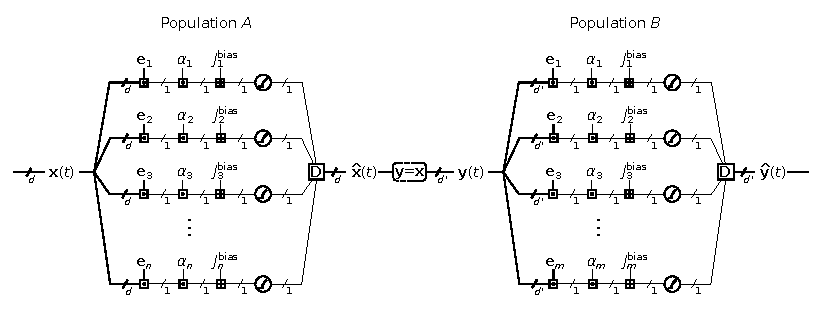
\includegraphics[width=\textwidth]{media/transformation_04.pdf}
		\caption{Illustration of the process of encoding and decoding values represented in two populations of neurons. If we wanted to build a communication channel without taking biology into account, we could just decode the value represented in population $A$ and then re-encode it in population $B$.}
		\label{fig:transformation_04}
	\end{figure}
	
	\begin{figure}[p]
		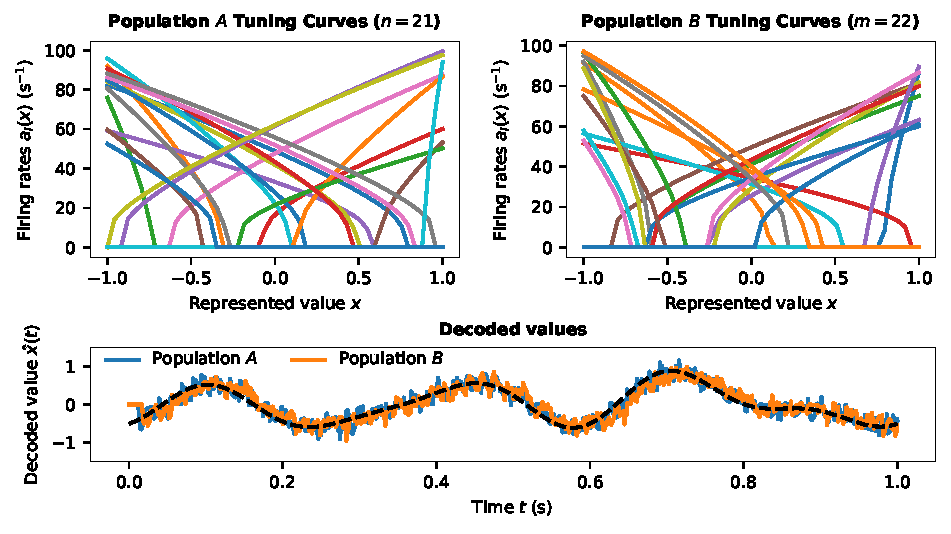
\includegraphics[width=\textwidth]{media/two_populations_decoding_series.pdf}
		\caption{Experiment depicting the effect of sequential decoding and re-encoding. \emph{Top:} tuning curves of the two neural populations. \emph{Bottom:} Representations decoded from population $A$ and $B$. The decoded output from $A$ is fed as an input into the population $B$.  Notice that the represented value is minimally delayed in population $B$.}
		\label{fig:two_populations_decoding_series}
	\end{figure}
	
	Given what we know so far, the simplest way of building a communication channel is by sequential encoding and decoding. We are decoding the value $\hat{\vec x}$ represented by a population $A$, followed by subsequent re-encoding of that value as $\vec y$, the value represented by population $B$. \Cref{fig:transformation_04} depicts the overall setup, including the individual encoding stages, neural nonlinearity and the decoder.
	
	An example of this type of communication channel is depicted in \cref{fig:two_populations_decoding_series}. As we can see, sequential decoding and re-encoding to transfer to the represented value from population $A$ to population $B$ seems to work, although there is a slight time delay between the two populations due to the synaptic filters.

	\Note{\emph{Location of the synaptic filter.} Notice that the synaptic filters $h$ are missing in \cref{fig:transformation_04}. In biology, the synaptic filter would be placed at each individual connection from a pre-neuron to a post-neuron (see below).
		
	However, since we assume that $h$ is a linear filter (this is because we model the filter using convolution) and that it has a \emph{unit DC gain}, placement of the filter does -- mathematically speaking -- not matter as long as it is placed before the nonlinearity of each neuron layer.}

	\subsection{Synaptic Weights}

	\begin{figure}
		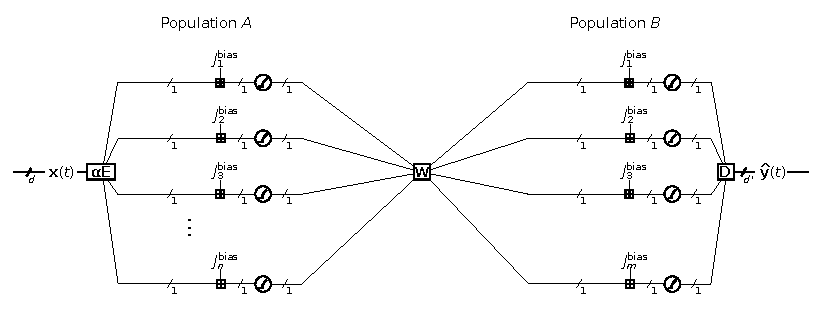
\includegraphics[width=\textwidth]{media/transformation_07.pdf}
		\caption{In biology, there are no encoders and decoders -- individual neurons are connected via synapse, and we model each synapse as a synaptic weight $w_{ij}$ (where $i$ is the post-neuron index, and $j$ is the pre-neuron index). We arrange these weights in a matrix $\big(\mat W \big)_{ij} = w_{ij}$}
	\end{figure}
	
	Evidently, the method discussed above works. Unfortunately, it is biologically implausible. While neurons are often characterised as belonging to different \enquote{populations} or \enquote{layers}, there is no equivalent of a dedicated decoder and encoder in biological neural networks that somehow translates between these layers. Instead, as we have discussed in previous lectures, individual neurons are connected via \emph{synapses}.
	
	Typically, there is an individual synapse for each connection from a pre-neuron $j$ to a post-neuron $i$. Mathematically, we model synapses as having two properties: a synaptic weight $w_{ij}$, as well as a synaptic filter $h$. The filter $h$ describes the translation from a pre-neuron spike into a post-synaptic current, whereas the weight $w_{ij}$ determines the magnitude of the current. Notice that we can arrange the synaptic weights $w_{ij}$ into a matrix $\mat W \in \mathbb{R}^{m \times n}$.

	We can categorize synaptic weights $w_{ij}$ into three different types:
	\begin{itemize}
		\item\textbf{Excitatory synapses $w_{ij} > 0$:}
		Excitatory synapses are characterized by evoking a positive post-synaptic current. That is, a spike from a pre-neuron arriving at an excitatory synapse will, on average, increase the firing rate of the post-neuron.
		\item\textbf{Inhibitory synapses $w_{ij} < 0$:}
		Conversely, inhibitory synapses are characterized by evoking a negative post-synaptic current. Spikes arriving at inhibitory synapses will decrease the average firing rate of the post-neuron.
		\item\textbf{No connection $w_{ij} = 0$:}
		By writing down a connection weight matrix $\mat W$, we implicitly assume that there is all-to-all connectivity between two populations of neurons. However, if a synaptic weights $w_{ij}$ happens to be exactly zero, this is equivalent to there being no connection between the pre-neuron $j$ and the post-neuron $i$.
	\end{itemize}

	\Note{\emph{Synaptic filters and synaptic weights.}
	Notice that we could collapse the synaptic weight $w_{ij}$ into the synaptic filter. In other words, instead of assuming that all synapses have the same synaptic filter, we could assign a scaled version of $h$ to each synapse, resulting in synaptic filters $h_{ij} = w_{ij} h$.

	The reason why we are not building our model in this way is solely due to computational complexity. By assuming that all synapses have the same synaptic filter $h$, we can (as mentioned in the previous note) exploit the linearity of convolution and collapse all convolutions into a single one.}

	\subsection{Synapse Models and Biological Correlates}

	As noted above, the synaptic weights $w_{ij}$, as well as the presence of a synaptic filter $h$, are integral parts of a synapse \emph{model}. That is, these two properties are a high-level abstraction of what is actually happening in biology.

	In particular, the synapse model $h$ summarizes the mechanisms that result in the distinct shape of the post-synaptic current, whereas the magnitude of the post-synaptic current is summarized in the weights $w_{ij}$. In biology, the magnitude of the response is influenced by a multitude of factors.
	\begin{itemize}
		\item \textbf{Presence of a synapse.}
		      If there is no connection between two neurons, the magnitude of the response, and thus $w_{ij}$, is zero.
		\item \textbf{Neurotransmitter type.}
		      The type of neurotransmitter emitted by the pre-synapse determines whether the post-synaptic current is excitatory or inhibitory. In biology, each neuron can only produce one kind of neurotransmitter, a fact known as \emph{Dale's principle} \cite{strata1999dale}. Correspondingly, neurons themselves act (in most cases) either excitatorily \emph{or} inhibitorily on the post-neuron.
		\item \textbf{Synaptic physiology.}
		      Among other factors, the number of synaptic vesicles, amount of neurotransmitter within a vesicle, number of receptors in the post synapse, determine the magnitude of the response.
		      
		      Furthermore, a pre-neuron may connect to the same post-neuron multiple times. As an extreme example of this, consider individual neurons in the Inferior Olive of the cerebellum, which connect to Purkinje cells via axons called \enquote{climbing fibres}. Surprisingly, each Inferior Olive neuron connects to \emph{exactly} one Purkinje cell, yet it does thousands of times.

		      Note that these properties can change over time, essentially modulating the synaptic weights; these longer-term changes in synaptic physiology are exactly what we refer to as the aforementioned \emph{learning}.
	\end{itemize}
	
	\Note{\emph{Current-based synapses.} In case we define our filter $h$ as follows
	\begin{align*}
		h(t) &= \begin{cases}
			\frac{1}{\tau} e^{-t / \tau} & \text{if } t \geq 0 \,,\\
			0 & \text{otherwise} \,,
		\end{cases}
	\end{align*}
	the specific synapse model we are using here is commonly referred to as a \enquote{current-based synapse model with exponential decay}. \enquote{Current-based} because we assume that synapses directly translate spikes into synaptic currents, \enquote{exponential decay} because of the form of the synaptic filter~\cite{roth2009modeling}.
	
	Of course, far more complex synapse models exist. We are going to talk about some of those -- in particular \emph{conductance-based} synapses (not to be confused with conductance-based neuron models, such as the Hodgkin Huxley model) -- in more detail when we talk about incorporating more biological realism into the Neural Engineering Framework.}

	\subsection{Computing Synaptic Weights}

	We now know that our previous approach -- sequential decoding and re-encoding -- works, but is biologically implausible because it does not describe neural connectivity in terms of synaptic weights $w_{ij}$. However, looking at the underlying equations we will see that this is not really true, and that we can in fact continue to use decoding and re-encoding as a mathematical abstraction.

	Combining the current-encoding equation from \cref{eqn:current} with the decoding equation from \cref{eqn:decoding}, we can write current that is being injected into the $i$-th neuron of the post-poulation as part of the decoding and re-encoding process as
	\begin{align*}
		J_i &= \alpha_i \langle \vec e_i, \mat D \vec a(\vec x) \rangle + J^\mathrm{bias}_i \,.
	\end{align*}
	Where $\vec a(\vec x)$ is the activity of the pre-population and $\mat D$ is the identity decoder of the pre-population. Expanding the scalar product and rearranging we get
	\begin{align*}
		J_i &= \alpha_i \sum_{k=1}^d e_{ik} \sum_{j=1}^n d_{kj} a_j(\vec x) + J^\mathrm{bias}_i
		     = \alpha_i \sum_{k=1}^d \sum_{j=1}^n e_{ik} d_{kj} a_j(\vec x) + J^\mathrm{bias}_i \\
		    &= \sum_{j=1}^n \underbrace{\alpha_i  \sum_{k=1}^d e_{ik} d_{kj}}_{w_{ij}} a_j(\vec x) + J^\mathrm{bias}_i
		     = \sum_{j=1}^n w_{ij} a_j(\vec x) + J^\mathrm{bias}_i \,.
	\end{align*}
	That is, we have now re-written the post-current of neuron $i$ purely in terms of a weighted sum of the pre-activities and a bias current. The coefficients $w_{ij}$ can be interpreted as exactly the weights we have been looking for.

	\begin{figure}
		\centering
		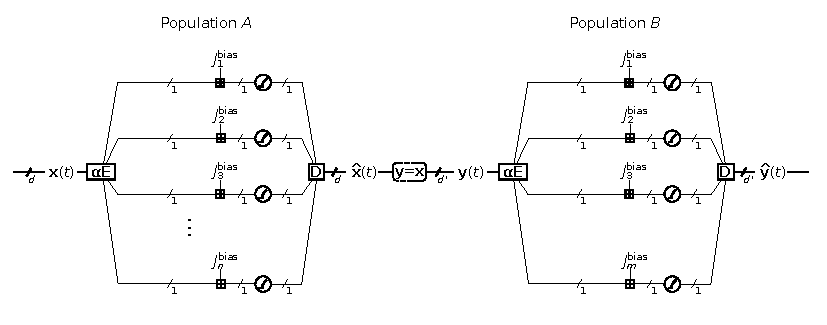
\includegraphics[width=\textwidth]{media/transformation_06.pdf}
		\caption{Decoding and encoding as linear operators. We can rearrange the linear parts of the encoding process into an encoding matrix $\mat E$.}
		\label{fig:transformation_06}
	\end{figure}
	Comparing \cref{fig:transformation_04} to \cref{fig:transformation_06} provides an alternative view on the above equations. Essentially, we can collapse the linear parts of the encoding process (multiplication with the encoding vectors $\vec e_i$ and scaling by $\alpha_i$) into a single matrix $\mat E$. We then have two chained linear operators, described by the decoding matrix $\mat D$ and the encoding matrix $\mat E$. The synaptic weight matrix $\mat W$ is then given as the product between the two, that is $\mat W = \mat E \mat D$.
	
	Using these synaptic weights $\mat W$ is hence \emph{mathematically equivalent} to sequential decoding and re-encoding. Whenever we want to have access to the biologically plausible synaptic weights we can just compute $\mat E \mat D$; otherwise we can continue to use encoders and decoders.

	\Note{\emph{Low-rank matrices, factorization, and computational complexity.}
	There is a good reason why we should continue to use sequential decoding and re-encoding in our simulations of neurobiological systems: once again, this boils down to computational complexity.

	\begin{center}
		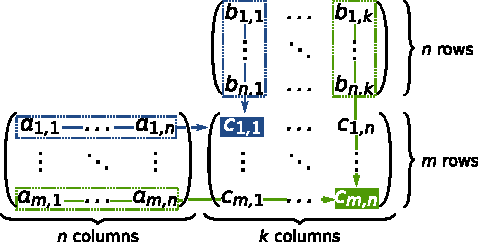
\includegraphics{media/matrix_multiplication_example.pdf}
	\end{center}
	The above figure illustrates the process of multiplying to matrices $\mat C = \mat A \mat B$, where $\mat A \in \mathbb{R}^{m\times n}$, $\mat B \in \mathbb{R}^{n \times k}$, and $\mat C \in \mathbb{R}^{m \times k}$. Na\"ively, each cell in $\mat C$ is the inner product between two vectors of size $n$. Since there are $m \times k$ cells in the matrix $\mat C$, the overall complexity is in $\mathcal{O}(m k n)$, or $\mathcal{O}(n^3)$ for the special case $m = k = n$. There are more clever, yet mostly impractical algorithms that (as of writing) bring the complexity down to $\mathcal{O}(n^{2.3728639})$ (see \href{https://en.wikipedia.org/wiki/Matrix\%20Multiplication\#Computational_complexity}{Wikipedia}).
	
	The computational complexity of multiplying the pre-population activities $\vec a \in \mathbb{R}^{n}$ with the weight matrix $\mat W \in \mathbb{R}^{m \times n}$ is hence $\mathcal{O}(n m)$, that is $\mathcal{O}(n^2)$ for the special case $n = m$.

	Conversely, assume that the dimensionality represented by the neuron populations $A$ and $B$ is $d$. The decoding process $\hat{\vec x} = \mat D \vec a$ has a computational complexity of $\mathcal{O}(d n)$, the encoding process $\vec J = \mat E \hat{\vec x} + \vec J_\mathrm{bias}$ has a complexity of $\mathcal{O}(d m)$. That makes for a total complexity of $\mathcal{O}(d (n + m))$, which is approximately $\mathcal{O}(d n)$ for $n = m$. Further assuming that $d$ is a small constant we get a linear complexity  $\mathcal{O}(n)$ for the sequential decoding and re-encoding process, compared to the quadratic complexity $\mathcal{O}(n^2)$ for the full weight matrix.

	Correspondingly, sequential decoding and re-encoding saves a lot of time compared to using actual synaptic weights, and is one of the reasons why Nengo is so fast compared to other spiking neural network simulators.

	This trick is a special case of a more general concept called \emph{matrix factorisation}. That is, matrix multiplication with a matrix $\mat A \in \mathbb{R}^{m \times k}$ is much faster if $\mat A$ can be decomposed -- or \emph{factorised} -- into the product of two smaller matrices $\mat A = \mat A_1 \mat A_2$, where $\mat A_1 \in \mathbb{R}^{m \times n}$ and $\mat A_2 \in \mathbb{R}^{n \times k}$, where the smallest possible $n$ for which such a product can be found is also called the \emph{rank} of a matrix. We can thus losslessly factorise a matrix and compute a fast matrix product if the matrix is of low rank, that is $n < \min \{m, k\}$.

%	\begin{align*}
%		&~ \begin{pmatrix}
%				b_{1, 1} & \ldots & b_{1, k} \\
%			\vdots & \ddots & \vdots \\
%			b_{n, 1} & \ldots & b_{n, k}
%		\end{pmatrix}\left.\vphantom{\begin{pmatrix}1\\2\\3\end{pmatrix}}\right\} {\scriptstyle n \text{ rows} }\\
%		\underbrace{\begin{pmatrix}
%			a_{1, 1} & \ldots & a_{1, n} \\
%			\vdots & \ddots & \vdots \\
%			a_{m, 1} & \ldots & a_{m, n}
%		\end{pmatrix}}_{n \text{ columns}} &~
%		\underbrace{\begin{pmatrix}
%			c_{1, 1} & \ldots & c_{1, n} \\
%			\vdots & \ddots & \vdots \\
%			c_{m, 1} & \ldots & c_{m, n}
%		\end{pmatrix}}_{k \text{ columns}}\left.\vphantom{\begin{pmatrix}1\\2\\3\end{pmatrix}}\right\} { \scriptstyle m \text{ rows} }
%	\end{align*}
	
	}

%´		\item $\mat W = \mat E \mat D$
%		\item $\mat W$ is of rank $d$. Computationally \emph{much} more efficient to decode and reencode!

	
	\section{Approximating Arbitrary Functions}

	Being able to build a communication channel using sequential decoding and re-encoding -- which, as we have discussed above, is equivalent to using a biologically plausible synaptic weight matrix $\mat W = \mat E \mat D$ -- does not seem to be particularly exciting. After all, we set out to compute arbitrary transformations $\vec y = f(\vec x)$. However, we are actually quite close to our goal.

	\subsection{Computing Linear Function Decoders}

	As a special case, let's first think about computing arbitrary linear transformations $f(\vec x) = \mat F \vec x$, where $\mat F \in \mathbb{R}^{d' \times d}$ transforms the $d$-dimensional value represented by the neural population $A$ into a $d'$-dimensional value that is going to be represented by the population $B$.

	Again, we can sequentially decode using $\mat D$, then apply our linear transformation $\mat F$, and finally re-encode the transformed value for the post-population using $\mat E$. All these operations being linear, we can just roll the linear transformation $\mat F$ into the decoder $\mat D$, giving us a specialised \emph{function decoder} $\mat D^{f} = \mat F \mat D \in \mathbb{R}^{d' \times n}$. Consequently, we could compute a synaptic weight matrix $\mat W^f = \mat E \mat D^f = \mat E \mat F \mat D$ that performs the desired transformation.

	\subsection{Computing Nonlinear Function Decoders}

	\begin{figure}
		\begin{subfigure}{\textwidth}
			\centering
			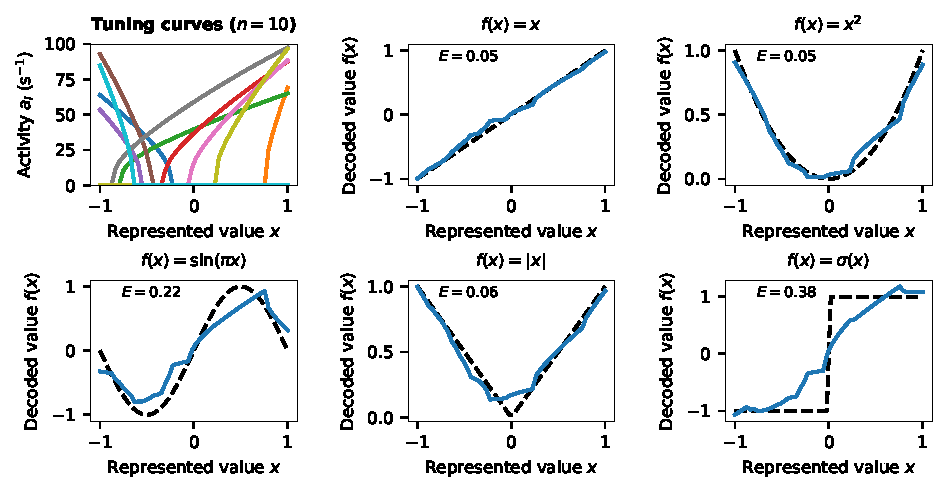
\includegraphics{media/function_decodings_10.pdf}
			\caption{Function decodings for $n = 10$ pre-synaptic neurons}
		\end{subfigure}\\[1cm]
		\begin{subfigure}{\textwidth}
			\centering
			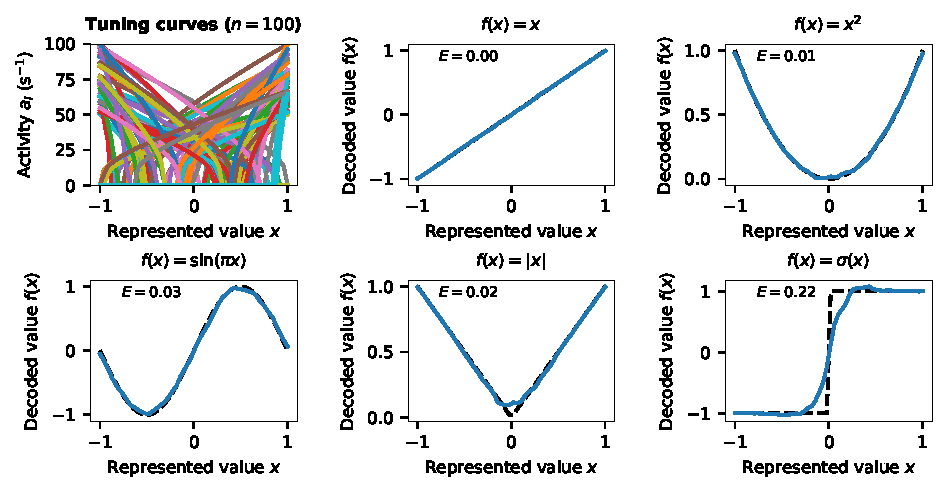
\includegraphics{media/function_decodings_100.pdf}
			\caption{Function decodings for $n = 100$ pre-synaptic neurons}
		\end{subfigure}
		\caption{Decoding arbitrary univariate functions $f$ from two neuron populations with different neuron counts $n$. The decoding error $E$ (depicted is the RMSE) decreases with the number of neurons, yet depends on the kind of function that is being computed. \CodeLink{lecture_05/media/code/function_decoding.ipynb}}
		\label{fig:function_decodings}
	\end{figure}

	We can generalise the above idea of a function decoder $\mat D^f$ to nonlinear functions. This can be accomplished by slightly adapting the optimization problem we are solving when computing the decoder. Instead of minimising the error $\| \hat{\vec x} - \vec x \|$ (where $\hat{\vec x} = \mat D \vec a(\vec x)$) over the space of represented values $\mathbb{X}$, we can minimise the error $\| \hat{\vec y} - f(\vec x) \|$, where $\hat{\vec y} = \mat D^f \vec a(\vec x)$:
	\begin{align*}
		\mat D^f &= \arg\min_{\mat D^f} \frac{1}{|\mathbb{X}|} \int_{\mathbb{X}} \big\| \mat D^f \vec a(\vec x) - f(\vec x) \big\|^2 \,\mathrm{d}{\vec x} \,.
	\end{align*}
	Note that this is essentially the same equation we were looking at when solving for the identity decoder -- the only difference being that $\vec x$ has been replaced by $f(\vec x) = \vec y$.

	As before, we can discretise the integral by sampling $N$ samples $\vec x_k \in \mathbb{X}$. Then, the function decoder $\mat D^f \in \mathbb{R}^{d' \times n}$ is given as
	\begin{ImportantEqn}{Function Decoder}
		\mat D^f = \left( (\mat A \mat A^\T + N \sigma^2 \mat I)^{-1} \mat A \mat Y^\T \right)^\T \,, \quad \text{where } \big ( \mat Y \big )_{ik} = \big( f(\vec x_k) \big)_i  \,.
	\end{ImportantEqn}
	Again, this is the same decoder computation equation as before. All we did is replacing the matrix $\mat X \in \mathbb{R}^{d \times N}$ by a matrix $\mat Y \in \mathbb{R}^{d' \times N}$, where each $\vec y_k = f(\vec x_k)$. In case $f(\vec x) = \vec x$ (the identity function), this method is \emph{exactly} equivalent to the equation we used to compute the identity decoder $\mat D$. \Cref{fig:function_decodings} shows some examples of various functions being decoded from a neural population. The quality of the function approximation depends on the number of pre-neurons, as well as the properties of the function we are trying to compute.
	\pagebreak
	\Note{\emph{Quality of function decodings.} When decoding a function $f$ from a neural population, we are only approximating that function -- the same way we were approximating the identity function when computing the identity decoder. Hence, we will see some error when computing transformations.
		
	As mentioned above, and as visible in \cref{fig:function_decodings}, the decoding error depends on the number of pre-neurons $n$ -- the more neurons, the smaller the error. Of course, when encoding the decoded value in the post-population, we are adding an representational error by representing the decoded value in a population of $m$ neurons.
	
	Furthermore, the error depends on the specific function $f$ we are trying to compute. In general, depending on the shape of the neural tuning curves, we can decode smooth, continuous functions quite well, whereas \enquote{jagged}, discontinuous functions are not well approximated by decoding from a population of neurons. We analyse why that is in a future lecture about analysing representations.}

	\subsection{Multiple Pre-Populations}

	\begin{figure}
		\centering%
		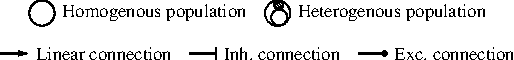
\includegraphics[scale=1.0]{media/network_legend_3.pdf}\\
		\begin{subfigure}{0.33\textwidth}%
			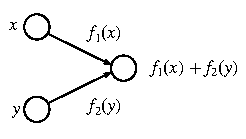
\includegraphics[scale=1.25]{media/network_a.pdf}%
			\caption{Linear combination of functions}
		\end{subfigure}%
		\begin{subfigure}{0.33\textwidth}%
			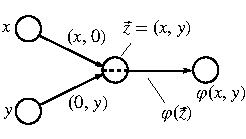
\includegraphics[scale=1.25]{media/network_c.pdf}%
			\caption{Computing nonlinear functions}
		\end{subfigure}%
		\begin{subfigure}{0.33\textwidth}%
			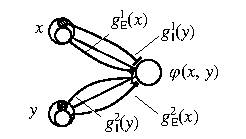
\includegraphics[scale=1.25]{media/network_d.pdf}%
			\caption{Dendritic computation}
		\end{subfigure}%
		\caption{Computing functions of values represented in multiple pre-populations. In general, if represented values are spread across multiple pre-populations, we can only compute linear combinations of functions of the represented values \textbf{(a)}. In order to compute nonlinear functions of multiple values, all values need to be represented in a higher-dimensional neuron population \textbf{(b)}. A special case is dendritic computation, where nonlinear effects within the synapses of a neuron are exploited in order to compute nonlinear multivariate functions of values not represented in the same pre-population.}
		\label{fig:network}
	\end{figure}
	
	We can now approximate arbitrary transformations $f(\vec x)$ in the connections between two neuron ensembles. Essentially, we just compute a function decoder $\mat D^f$ and then perform sequential decoding and re-encoding, which on demand can be turned into a biologically plausible neural network with a synaptic weight matrix $\mat W^f = \mat E \mat D^f$.

	The next question would be what happens if we connect multiple pre-populations to the same post-population. In the Neural Engineering Framework, we assume that we just sum the post-synaptic currents evoked by both pre-populations. Hence, the current $J_i$ flowing into the $i$-th pre-neuron is
	\begin{align*}
		J_i &= \langle \vec e_i, \mat D^f \vec a_1 \rangle + \langle \vec e_i, \mat D^g \vec a_2 \rangle + J^\mathrm{bias}_i \,,
	\end{align*}
	where $\vec a_1$ are the activities of the first pre-population, $\vec a_2$ are the activities of the second pre-population, $\mat D^f$ is a function decoder decoding $f$ from the first-propulation, and $\mat D^g$ decodes $g$ form the second pre-population. Note that we can rewrite the above equation as
	\begin{align*}
		J_i &= \langle \vec e_i, \mat D^f \vec a_1 + \mat D^g \vec a_2 \rangle + J^\mathrm{bias}_i \approx \langle \vec e_i, f(\vec x_1) + g(\vec x_2) \rangle \,,
	\end{align*}
	where $\vec x_1$ and $\vec x_2$ are the values represented by the two pre-populations. This means that we are essentially computing the sum of the two functions.

	Note that this does not allow us to compute non-linear multivariate functions such as $\varphi(x, y) = xy$, if $x$ and $y$ are represented in separate pre-populations. However, we can compute multiplication by representing $x$ and $y$ in a two-dimensional population representing $\vec z = (x, y)$, and then decode $\varphi$ out of this population (\cref{fig:network}).
	\printbibliography
	
\end{document}
